\documentclass[pdf]{beamer}
\mode<presentation>{}
\usepackage{colortbl}
\usepackage{tikz}
\usetikzlibrary{positioning}
\usetikzlibrary{arrows}
\usepackage[utf8]{inputenc}
\usepackage[T1]{fontenc}
\usepackage{mathtools}
\DeclarePairedDelimiter\ceil{\lceil}{\rceil}
\DeclarePairedDelimiter\floor{\lfloor}{\rfloor}

\setbeamertemplate{footline}[frame number]

%% preamble
\title{Tree data structures}
\author{Guillaume \textsc{Derval}}

\begin{document}

%% title frame
\begin{frame}
\titlepage
\end{frame}

{
\begin{frame}{Table of Contents}
\tableofcontents[]
\end{frame}
}

\AtBeginSection[]
{
\begin{frame}{Table of Contents}
\tableofcontents[currentsection]
\end{frame}
}

\AtBeginSubsection[]
{
\begin{frame}{Table of Contents}
\tableofcontents[currentsection, currentsubsection]
\end{frame}
}

\section{Binary Search Trees, Sets and Maps}

\begin{frame}
	\frametitle{Definition}
	A binary search tree ...
	\begin{itemize}
		\item is a tree ( :O )
		\item is binary ( :O ). So, two children maximum, that we name "left" and "right"
		\item such that each nodes stores a "key" and a "value" (which can be the same as the key)
		\item respects the "search property": 
		\begin{itemize}
			\item all nodes on the left subtree are $<$ the current node
			\item all nodes on the right subtree are $>$ the current node
		\end{itemize}
	\end{itemize}
\end{frame}

\begin{frame}
	\frametitle{Invalid BST example}
	
	\begin{center}
		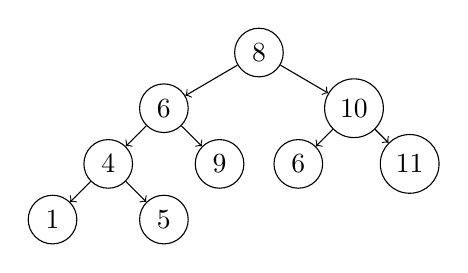
\begin{tikzpicture}[->,nodes={draw, circle}]
		\node (a8) [] {8};
		\node (a6) [below left of = a8, xshift=-0.5cm] {6};
		\node (a10) [below right of = a8, xshift=0.5cm]{10};
		\node (a4) [below left of = a6]{4};
		\node (a7) [below right of = a6]{9};
		\node (a9) [below left of = a10]{6};
		\node (a11) [below right of = a10]{11};
		\node (a1) [below left of = a4]{1};
		\node (n7) [below right of = a4]{5};
		\draw (a8) -> (a10);
		\draw (a8) -> (a6); 
		\draw (a6) -> (a4);
		\draw (a6) -> (a7);
		\draw (a10) -> (a9);
		\draw (a10) -> (a11);
		\draw (a4) -> (a1);
		\draw (a4) -> (n7);
		\end{tikzpicture}
	\end{center}
\end{frame}

\begin{frame}
	\frametitle{BST example}
	
	\begin{center}
		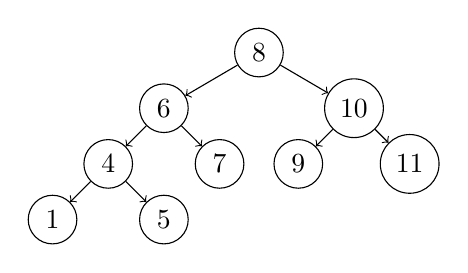
\begin{tikzpicture}[->,nodes={draw, circle}]
		\node (a8) [] {8};
		\node (a6) [below left of = a8, xshift=-0.5cm] {6};
		\node (a10) [below right of = a8, xshift=0.5cm]{10};
		\node (a4) [below left of = a6]{4};
		\node (a7) [below right of = a6]{7};
		\node (a9) [below left of = a10]{9};
		\node (a11) [below right of = a10]{11};
		\node (a1) [below left of = a4]{1};
		\node (n7) [below right of = a4]{5};
		\draw (a8) -> (a10);
		\draw (a8) -> (a6); 
		\draw (a6) -> (a4);
		\draw (a6) -> (a7);
		\draw (a10) -> (a9);
		\draw (a10) -> (a11);
		\draw (a4) -> (a1);
		\draw (a4) -> (n7);
		\end{tikzpicture}
	\end{center}
\end{frame}

\begin{frame}
	\frametitle{Balanced Search Tree}
	A (binary) tree is said to be balanced if its height is minimal, that is if its height is $\floor{\log_2(n)}$
	
	Most the of the BST are balanced. We will see later why...
\end{frame}

\begin{frame}
	\frametitle{Common operations}
	\begin{itemize}
		\item search(key): returns the value associated with the key
		\item insert(key, value): insert a new key/value
		\item findMax(): returns the key/value associated with the biggest key
		\item findMin(): ...
		\item successor(key): returns the key/value immediately after the given key
		\item predecessor(key): ...
	\end{itemize}
\end{frame}

\begin{frame}
	\frametitle{Implementing search operations}
	Let's say we want to find the value associated with $5$ in this tree:
	
	\begin{center}
		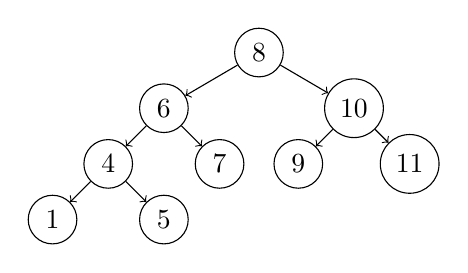
\begin{tikzpicture}[->,nodes={draw, circle}]
		\node (a8) [] {8};
		\node (a6) [below left of = a8, xshift=-0.5cm] {6};
		\node (a10) [below right of = a8, xshift=0.5cm]{10};
		\node (a4) [below left of = a6]{4};
		\node (a7) [below right of = a6]{7};
		\node (a9) [below left of = a10]{9};
		\node (a11) [below right of = a10]{11};
		\node (a1) [below left of = a4]{1};
		\node (n7) [below right of = a4]{5};
		\draw (a8) -> (a10);
		\draw (a8) -> (a6); 
		\draw (a6) -> (a4);
		\draw (a6) -> (a7);
		\draw (a10) -> (a9);
		\draw (a10) -> (a11);
		\draw (a4) -> (a1);
		\draw (a4) -> (n7);
		\end{tikzpicture}
	\end{center}
\end{frame}

\begin{frame}
	\frametitle{Implementing search operations}
	Let's start at the root:
	
	\only<2>{8 > 5: search only on the left}
	
	\begin{center}
		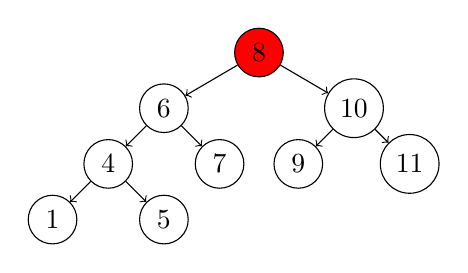
\begin{tikzpicture}[->,nodes={draw, circle}]
		\node (a8) [fill=red] {8};
		\node (a6) [below left of = a8, xshift=-0.5cm] {6};
		\node (a10) [below right of = a8, xshift=0.5cm]{10};
		\node (a4) [below left of = a6]{4};
		\node (a7) [below right of = a6]{7};
		\node (a9) [below left of = a10]{9};
		\node (a11) [below right of = a10]{11};
		\node (a1) [below left of = a4]{1};
		\node (n7) [below right of = a4]{5};
		\draw (a8) -> (a10);
		\draw (a8) -> (a6); 
		\draw (a6) -> (a4);
		\draw (a6) -> (a7);
		\draw (a10) -> (a9);
		\draw (a10) -> (a11);
		\draw (a4) -> (a1);
		\draw (a4) -> (n7);
		\end{tikzpicture}
	\end{center}
\end{frame}

\begin{frame}
	\frametitle{Implementing search operations}
	We are now at 6
	
	\only<2>{6 > 5: search only on the left}
	
	\begin{center}
		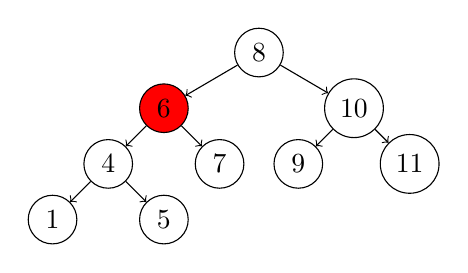
\begin{tikzpicture}[->,nodes={draw, circle}]
		\node (a8) [] {8};
		\node (a6) [below left of = a8, xshift=-0.5cm, fill=red] {6};
		\node (a10) [below right of = a8, xshift=0.5cm]{10};
		\node (a4) [below left of = a6]{4};
		\node (a7) [below right of = a6]{7};
		\node (a9) [below left of = a10]{9};
		\node (a11) [below right of = a10]{11};
		\node (a1) [below left of = a4]{1};
		\node (n7) [below right of = a4]{5};
		\draw (a8) -> (a10);
		\draw (a8) -> (a6); 
		\draw (a6) -> (a4);
		\draw (a6) -> (a7);
		\draw (a10) -> (a9);
		\draw (a10) -> (a11);
		\draw (a4) -> (a1);
		\draw (a4) -> (n7);
		\end{tikzpicture}
	\end{center}
\end{frame}

\begin{frame}
	\frametitle{Implementing search operations}
	We are now at 4
	
	\only<2>{4 < 5: search only on the right}
	
	\begin{center}
		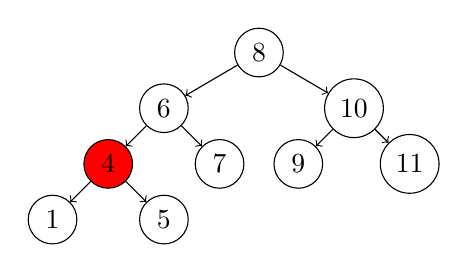
\begin{tikzpicture}[->,nodes={draw, circle}]
		\node (a8) [] {8};
		\node (a6) [below left of = a8, xshift=-0.5cm] {6};
		\node (a10) [below right of = a8, xshift=0.5cm]{10};
		\node (a4) [below left of = a6, fill=red]{4};
		\node (a7) [below right of = a6]{7};
		\node (a9) [below left of = a10]{9};
		\node (a11) [below right of = a10]{11};
		\node (a1) [below left of = a4]{1};
		\node (n7) [below right of = a4]{5};
		\draw (a8) -> (a10);
		\draw (a8) -> (a6); 
		\draw (a6) -> (a4);
		\draw (a6) -> (a7);
		\draw (a10) -> (a9);
		\draw (a10) -> (a11);
		\draw (a4) -> (a1);
		\draw (a4) -> (n7);
		\end{tikzpicture}
	\end{center}
\end{frame}

\begin{frame}
	\frametitle{Implementing search operations}
	We are now at 5. Return the key/value pair.
	
	\begin{center}
		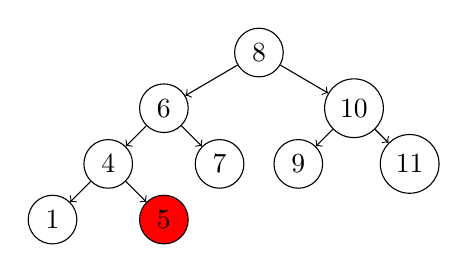
\begin{tikzpicture}[->,nodes={draw, circle}]
		\node (a8) [] {8};
		\node (a6) [below left of = a8, xshift=-0.5cm] {6};
		\node (a10) [below right of = a8, xshift=0.5cm]{10};
		\node (a4) [below left of = a6]{4};
		\node (a7) [below right of = a6]{7};
		\node (a9) [below left of = a10]{9};
		\node (a11) [below right of = a10]{11};
		\node (a1) [below left of = a4]{1};
		\node (n7) [below right of = a4, fill=red]{5};
		\draw (a8) -> (a10);
		\draw (a8) -> (a6); 
		\draw (a6) -> (a4);
		\draw (a6) -> (a7);
		\draw (a10) -> (a9);
		\draw (a10) -> (a11);
		\draw (a4) -> (a1);
		\draw (a4) -> (n7);
		\end{tikzpicture}
	\end{center}
\end{frame}

\begin{frame}
	\frametitle{Complexity?}
	\pause $O(\text{height of the tree})$
	\pause $= O(\floor{\log(n)})$ if the tree is balanced
	\vspace{2cm}
	\pause Without a balanced tree, all the operations are $O(n)$!
\end{frame}

\begin{frame}
	\frametitle{Implementing a balanced BST}
	Ideas?
\end{frame}

\begin{frame}
	\frametitle{Implementing a balanced BST}
	\begin{figure}
		\centering
		\includegraphics[width=0.7\linewidth]{toohard}
	\end{figure}
\end{frame}

\begin{frame}
	\frametitle{Implementing a balanced BST}
	\begin{figure}
		\centering
		\includegraphics[width=0.7\linewidth]{time}
	\end{figure}
	
	\begin{itemize}
		\pause\item Too complicated to explain right now
		\pause\item Too complicated to remember
		\pause\item Too long to implement during a contest
		\pause\item Very prone to bugs
	\end{itemize}
	Still, if you have time, it's very interesting to know, but won't be useful during competitive programming contests
\end{frame}

\begin{frame}
	\frametitle{Use the STL}
	(real) languages come with implementations of BST, in two categories
	\begin{itemize}
		\item Sets: represents a mathematical set. It is, in fact, a BST with keys==values
			\begin{itemize}
				\item C++: std::set
				\item Java: TreeSet
			\end{itemize}
		\item Maps: dictionnary
		\begin{itemize}
			\item C++: std::map
			\item Java: TreeMap
		\end{itemize}
	\end{itemize}
\end{frame}
\section{Heap}

\begin{frame}
	\frametitle{Heap}
	A heap is a structure with (mainly) two operations:
	\begin{itemize}
		\item \texttt{push}: Add an element to the heap $O(\log n)$.
		\item \texttt{pop}: remove and return the biggest/greater/... element from the heap $O(\log n)$.
	\end{itemize}
	\pause How to implement it?
	\pause With a tree, of course!
\end{frame}

\begin{frame}
	\frametitle{The heap property}
	Remember the binary search tree property?\\
	\vspace{1cm}
	\textbf{(max) Heap property}: Childrens of a node in a heap tree are $\leq$ than the node itself.\\
	\vspace{1cm}
	One of the most simple and efficient heap implementation are complete binary heap. Two more rules then:
	\begin{itemize}
		\item The tree is a binary one ($\leq$ 2 children per node)
		\item The tree is "complete": all levels of the tree are full of nodes but the last one, on which leaves are on the left
	\end{itemize}
\end{frame}


\begin{frame}
	\frametitle{Which are valid complete binary heap trees?}
	
	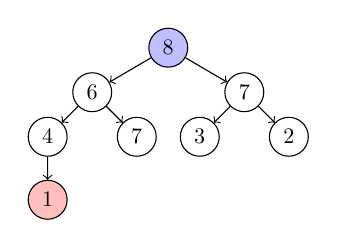
\begin{tikzpicture}[->,nodes={draw, circle,scale=0.8},scale=0.8]
	\node (a8) [fill = blue!25] {8};
	\node (a6) [below left of = a8, xshift=-0.5cm] {6};
	\node (a7) [below right of = a8, xshift=0.5cm]{7};
	\node (a4) [below left of = a6]{4};
	\node (a5) [below right of = a6]{7};
	\node (a3) [below left of = a7]{3};
	\node (a2) [below right of = a7]{2};
	\node (a1) [below of = a4, fill = red!25]{1};
	
	\draw (a8) -> (a7);
	\draw (a8) -> (a6); 
	\draw (a6) -> (a4);
	\draw (a6) -> (a5);
	\draw (a7) -> (a3);
	\draw (a7) -> (a2);
	\draw (a4) -> (a1);
	\end{tikzpicture} \only<2>{(heap property not respected on 6-7)}
	
	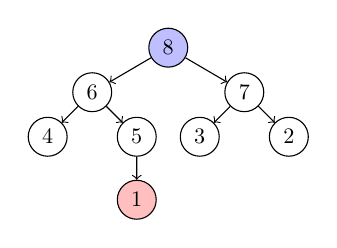
\begin{tikzpicture}[->,nodes={draw, circle,scale=0.8},scale=0.8]
	\node (a8) [fill = blue!25] {8};
	\node (a6) [below left of = a8, xshift=-0.5cm] {6};
	\node (a7) [below right of = a8, xshift=0.5cm]{7};
	\node (a4) [below left of = a6]{4};
	\node (a5) [below right of = a6]{5};
	\node (a3) [below left of = a7]{3};
	\node (a2) [below right of = a7]{2};
	\node (a1) [below of = a5, fill = red!25]{1};
	
	\draw (a8) -> (a7);
	\draw (a8) -> (a6); 
	\draw (a6) -> (a4);
	\draw (a6) -> (a5);
	\draw (a7) -> (a3);
	\draw (a7) -> (a2);
	\draw (a5) -> (a1);
	\end{tikzpicture} \only<2>{(leaf 1 not on left)}
	
	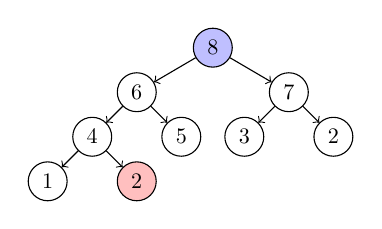
\begin{tikzpicture}[->,nodes={draw, circle,scale=0.8},scale=0.8]
	\node (a8) [fill = blue!25] {8};
	\node (a6) [below left of = a8, xshift=-0.5cm] {6};
	\node (a7) [below right of = a8, xshift=0.5cm]{7};
	\node (a4) [below left of = a6]{4};
	\node (a5) [below right of = a6]{5};
	\node (a3) [below left of = a7]{3};
	\node (a2) [below right of = a7]{2};
	\node (a1) [below left of = a4]{1};
	\node (a22) [below right of = a4, fill = red!25]{2};
	
	\draw (a8) -> (a7);
	\draw (a8) -> (a6); 
	\draw (a6) -> (a4);
	\draw (a6) -> (a5);
	\draw (a7) -> (a3);
	\draw (a7) -> (a2);
	\draw (a4) -> (a1);
	\draw (a4) -> (a22);
	\end{tikzpicture} \only<2>{(valid!)}
\end{frame}

\begin{frame}
	\frametitle{Storing a complete tree}
	Storing a complete tree is easy: use an array (or a vector)!
	\vspace{0.5cm}
	\begin{center}
		\begin{tabular}{ccccccccc}
			0 & 1 & 2 & 3 & 4 & 5 & 6 & 7 & 8\\
		\end{tabular}
		\begin{tabular}{|c|c|c|c|c|c|c|c|c|}
			\hline
			a & b & c & d & e & f & g & h & i\\
			\hline
		\end{tabular}
		
		\vspace{0.5cm}
		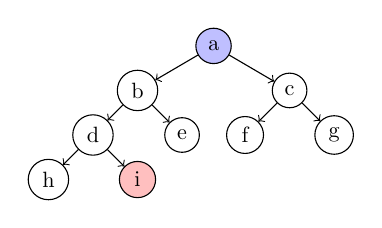
\begin{tikzpicture}[->,nodes={draw, circle,scale=0.8},scale=0.8]
		\node (a8) [fill = blue!25] {a};
		\node (a6) [below left of = a8, xshift=-0.5cm] {b};
		\node (a7) [below right of = a8, xshift=0.5cm]{c};
		\node (a4) [below left of = a6]{d};
		\node (a5) [below right of = a6]{e};
		\node (a3) [below left of = a7]{f};
		\node (a2) [below right of = a7]{g};
		\node (a1) [below left of = a4]{h};
		\node (a22) [below right of = a4, fill = red!25]{i};
		
		\draw (a8) -> (a7);
		\draw (a8) -> (a6); 
		\draw (a6) -> (a4);
		\draw (a6) -> (a5);
		\draw (a7) -> (a3);
		\draw (a7) -> (a2);
		\draw (a4) -> (a1);
		\draw (a4) -> (a22);
		\end{tikzpicture}
	\end{center}
	If $p$ is the idx of the parent in the array, idx of the children are:
	\begin{itemize}
		\item $2p+1$
		\item $2p+2$
	\end{itemize}
	Next node to be created is always at the end of the array!
\end{frame}

\begin{frame}
	\frametitle{Adding a new element}
	\begin{enumerate}
		\item Add new element at the end of the tree
		\item If parent does not respect the heap property (== is lesser than the new node)
		\begin{enumerate}
			\item Exchange the node and its parent
			\item Repeat from 2.
		\end{enumerate}
	\end{enumerate}
\end{frame}

\begin{frame}
	\frametitle{Adding a new element}
	Adding $7$:
	\begin{center}
	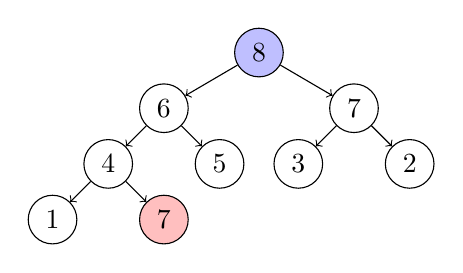
\begin{tikzpicture}[->,nodes={draw, circle}]
	\node (a8) [fill = blue!25] {8};
	\node (a6) [below left of = a8, xshift=-0.5cm] {6};
	\node (a7) [below right of = a8, xshift=0.5cm]{7};
	\node (a4) [below left of = a6]{4};
	\node (a5) [below right of = a6]{5};
	\node (a3) [below left of = a7]{3};
	\node (a2) [below right of = a7]{2};
	\node (a1) [below left of = a4]{1};
	\node (n7) [below right of = a4, fill = red!25]{7};
	\draw (a8) -> (a7);
	\draw (a8) -> (a6); 
	\draw (a6) -> (a4);
	\draw (a6) -> (a5);
	\draw (a7) -> (a3);
	\draw (a7) -> (a2);
	\draw (a4) -> (a1);
	\draw (a4) -> (n7);
	\end{tikzpicture}
	\end{center}
\end{frame}

\begin{frame}
	\frametitle{Adding a new element}
	Adding $7$:
	\begin{center}
		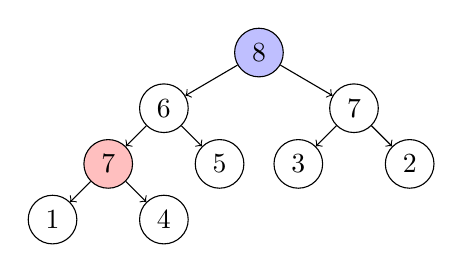
\begin{tikzpicture}[->,nodes={draw, circle}]
		\node (a8) [fill = blue!25] {8};
		\node (a6) [below left of = a8, xshift=-0.5cm] {6};
		\node (a7) [below right of = a8, xshift=0.5cm]{7};
		\node (a4) [below left of = a6, fill = red!25]{7};
		\node (a5) [below right of = a6]{5};
		\node (a3) [below left of = a7]{3};
		\node (a2) [below right of = a7]{2};
		\node (a1) [below left of = a4]{1};
		\node (n7) [below right of = a4]{4};
		\draw (a8) -> (a7);
		\draw (a8) -> (a6); 
		\draw (a6) -> (a4);
		\draw (a6) -> (a5);
		\draw (a7) -> (a3);
		\draw (a7) -> (a2);
		\draw (a4) -> (a1);
		\draw (a4) -> (n7);
		\end{tikzpicture}
	\end{center}
\end{frame}

\begin{frame}
	\frametitle{Adding a new element}
	Adding $7$:
	\begin{center}
		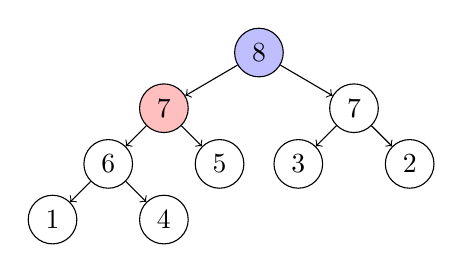
\begin{tikzpicture}[->,nodes={draw, circle}]
		\node (a8) [fill = blue!25] {8};
		\node (a6) [below left of = a8, xshift=-0.5cm, fill = red!25] {7};
		\node (a7) [below right of = a8, xshift=0.5cm]{7};
		\node (a4) [below left of = a6]{6};
		\node (a5) [below right of = a6]{5};
		\node (a3) [below left of = a7]{3};
		\node (a2) [below right of = a7]{2};
		\node (a1) [below left of = a4]{1};
		\node (n7) [below right of = a4]{4};
		\draw (a8) -> (a7);
		\draw (a8) -> (a6); 
		\draw (a6) -> (a4);
		\draw (a6) -> (a5);
		\draw (a7) -> (a3);
		\draw (a7) -> (a2);
		\draw (a4) -> (a1);
		\draw (a4) -> (n7);
		\end{tikzpicture}
	\end{center}
\end{frame}

\begin{frame}
	\frametitle{Adding a new element}
	Adding $7$:
	\begin{center}
		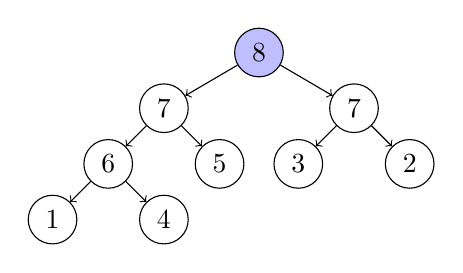
\begin{tikzpicture}[->,nodes={draw, circle}]
		\node (a8) [fill = blue!25] {8};
		\node (a6) [below left of = a8, xshift=-0.5cm] {7};
		\node (a7) [below right of = a8, xshift=0.5cm]{7};
		\node (a4) [below left of = a6]{6};
		\node (a5) [below right of = a6]{5};
		\node (a3) [below left of = a7]{3};
		\node (a2) [below right of = a7]{2};
		\node (a1) [below left of = a4]{1};
		\node (n7) [below right of = a4]{4};
		\draw (a8) -> (a7);
		\draw (a8) -> (a6); 
		\draw (a6) -> (a4);
		\draw (a6) -> (a5);
		\draw (a7) -> (a3);
		\draw (a7) -> (a2);
		\draw (a4) -> (a1);
		\draw (a4) -> (n7);
		\end{tikzpicture}
	\end{center}
\end{frame}

\begin{frame}
	\frametitle{Removing the first element}
	\begin{enumerate}
		\item Save somewhere the root of the tree to return it later
		\item Take the last node value, and put it at the top of the tree
		\item Three cases then:
			\begin{itemize}
				\item If the heap property is respected (node $\geq$ its children), return
				\item If one of the children is $>$ the node, swap them and repeat from 3.
				\item If both children are $>$ the node, swap with the greatest child and repeat from 3.
			\end{itemize}
	\end{enumerate}
\end{frame}

\begin{frame}
	\frametitle{Removing the first element}
	Step 1: store the root somewhere (remember: root was 8)
	
	\begin{center}
		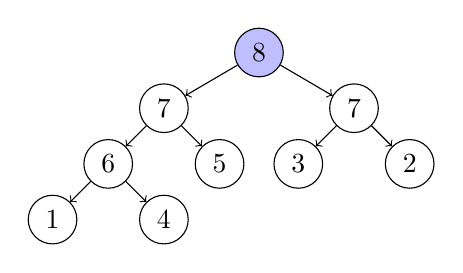
\begin{tikzpicture}[->,nodes={draw, circle}]
		\node (a8) [fill = blue!25] {8};
		\node (a6) [below left of = a8, xshift=-0.5cm] {7};
		\node (a7) [below right of = a8, xshift=0.5cm]{7};
		\node (a4) [below left of = a6]{6};
		\node (a5) [below right of = a6]{5};
		\node (a3) [below left of = a7]{3};
		\node (a2) [below right of = a7]{2};
		\node (a1) [below left of = a4]{1};
		\node (n7) [below right of = a4]{4};
		\draw (a8) -> (a7);
		\draw (a8) -> (a6); 
		\draw (a6) -> (a4);
		\draw (a6) -> (a5);
		\draw (a7) -> (a3);
		\draw (a7) -> (a2);
		\draw (a4) -> (a1);
		\draw (a4) -> (n7);
		\end{tikzpicture}
	\end{center}
\end{frame}

\begin{frame}
	\frametitle{Removing the first element}
	Step 2: put the last node at the root
	
	\begin{center}
		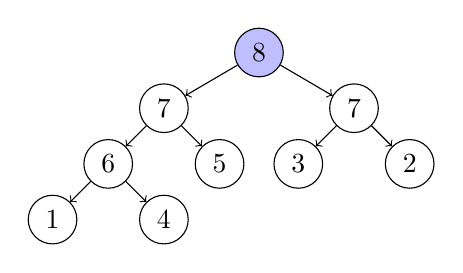
\begin{tikzpicture}[->,nodes={draw, circle}]
		\node (a8) [fill = blue!25] {8};
		\node (a6) [below left of = a8, xshift=-0.5cm] {7};
		\node (a7) [below right of = a8, xshift=0.5cm]{7};
		\node (a4) [below left of = a6]{6};
		\node (a5) [below right of = a6]{5};
		\node (a3) [below left of = a7]{3};
		\node (a2) [below right of = a7]{2};
		\node (a1) [below left of = a4]{1};
		\node (n7) [below right of = a4]{4};
		\draw (a8) -> (a7);
		\draw (a8) -> (a6); 
		\draw (a6) -> (a4);
		\draw (a6) -> (a5);
		\draw (a7) -> (a3);
		\draw (a7) -> (a2);
		\draw (a4) -> (a1);
		\draw (a4) -> (n7);
		\end{tikzpicture}
	\end{center}
\end{frame}

\begin{frame}
	\frametitle{Removing the first element}
	Step 2: put the last node at the root
	
	\begin{center}
		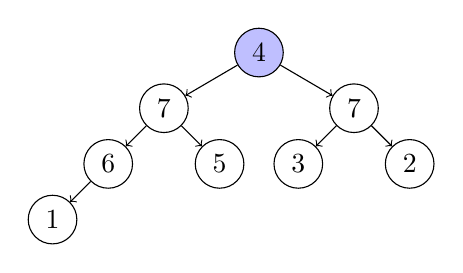
\begin{tikzpicture}[->,nodes={draw, circle}]
		\node (a8) [fill = blue!25] {4};
		\node (a6) [below left of = a8, xshift=-0.5cm] {7};
		\node (a7) [below right of = a8, xshift=0.5cm]{7};
		\node (a4) [below left of = a6]{6};
		\node (a5) [below right of = a6]{5};
		\node (a3) [below left of = a7]{3};
		\node (a2) [below right of = a7]{2};
		\node (a1) [below left of = a4]{1};
		\draw (a8) -> (a7);
		\draw (a8) -> (a6); 
		\draw (a6) -> (a4);
		\draw (a6) -> (a5);
		\draw (a7) -> (a3);
		\draw (a7) -> (a2);
		\draw (a4) -> (a1);
		\end{tikzpicture}
	\end{center}
\end{frame}

\begin{frame}
	\frametitle{Removing the first element}
	Step 3: check heap property with the children of the node.\\
	\only<2>{\textbf{Not respected -> swap with (the first) 7}}
	\begin{center}
		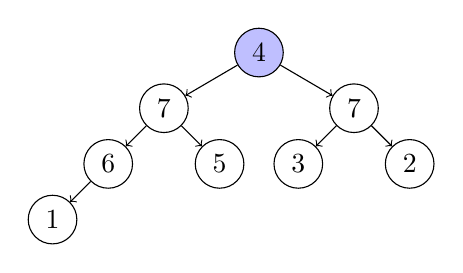
\begin{tikzpicture}[->,nodes={draw, circle}]
		\node (a8) [fill = blue!25] {4};
		\node (a6) [below left of = a8, xshift=-0.5cm] {7};
		\node (a7) [below right of = a8, xshift=0.5cm]{7};
		\node (a4) [below left of = a6]{6};
		\node (a5) [below right of = a6]{5};
		\node (a3) [below left of = a7]{3};
		\node (a2) [below right of = a7]{2};
		\node (a1) [below left of = a4]{1};
		\draw (a8) -> (a7);
		\draw (a8) -> (a6); 
		\draw (a6) -> (a4);
		\draw (a6) -> (a5);
		\draw (a7) -> (a3);
		\draw (a7) -> (a2);
		\draw (a4) -> (a1);
		\end{tikzpicture}
	\end{center}
\end{frame}

\begin{frame}
	\frametitle{Removing the first element}
	Step 3: check heap property with the children of the node.\\
	\textbf{Not respected -> swap with (the first) 7}
	\begin{center}
		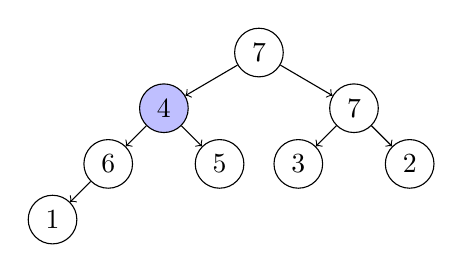
\begin{tikzpicture}[->,nodes={draw, circle}]
		\node (a8) [] {7};
		\node (a6) [below left of = a8, xshift=-0.5cm,fill = blue!25] {4};
		\node (a7) [below right of = a8, xshift=0.5cm]{7};
		\node (a4) [below left of = a6]{6};
		\node (a5) [below right of = a6]{5};
		\node (a3) [below left of = a7]{3};
		\node (a2) [below right of = a7]{2};
		\node (a1) [below left of = a4]{1};
		\draw (a8) -> (a7);
		\draw (a8) -> (a6); 
		\draw (a6) -> (a4);
		\draw (a6) -> (a5);
		\draw (a7) -> (a3);
		\draw (a7) -> (a2);
		\draw (a4) -> (a1);
		\end{tikzpicture}
	\end{center}
\end{frame}

\begin{frame}
	\frametitle{Removing the first element}
	Step 3: check heap property with the children of the node.\\
	\textbf{Not respected -> swap with 6 (the greatest child)}
	\begin{center}
		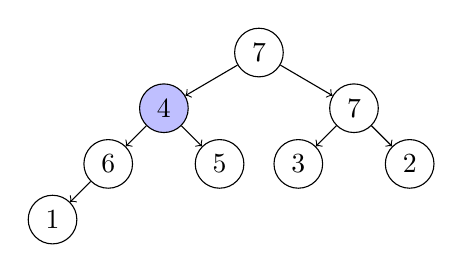
\begin{tikzpicture}[->,nodes={draw, circle}]
		\node (a8) [] {7};
		\node (a6) [below left of = a8, xshift=-0.5cm,fill = blue!25] {4};
		\node (a7) [below right of = a8, xshift=0.5cm]{7};
		\node (a4) [below left of = a6]{6};
		\node (a5) [below right of = a6]{5};
		\node (a3) [below left of = a7]{3};
		\node (a2) [below right of = a7]{2};
		\node (a1) [below left of = a4]{1};
		\draw (a8) -> (a7);
		\draw (a8) -> (a6); 
		\draw (a6) -> (a4);
		\draw (a6) -> (a5);
		\draw (a7) -> (a3);
		\draw (a7) -> (a2);
		\draw (a4) -> (a1);
		\end{tikzpicture}
	\end{center}
\end{frame}

\begin{frame}
	\frametitle{Removing the first element}
	Step 3: check heap property with the children of the node.\\
	\textbf{Not respected -> swap with 6 (the greatest child)}
	\begin{center}
		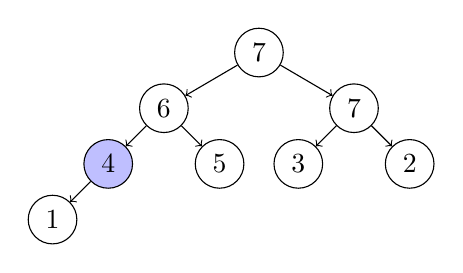
\begin{tikzpicture}[->,nodes={draw, circle}]
		\node (a8) [] {7};
		\node (a6) [below left of = a8, xshift=-0.5cm] {6};
		\node (a7) [below right of = a8, xshift=0.5cm]{7};
		\node (a4) [below left of = a6,fill = blue!25]{4};
		\node (a5) [below right of = a6]{5};
		\node (a3) [below left of = a7]{3};
		\node (a2) [below right of = a7]{2};
		\node (a1) [below left of = a4]{1};
		\draw (a8) -> (a7);
		\draw (a8) -> (a6); 
		\draw (a6) -> (a4);
		\draw (a6) -> (a5);
		\draw (a7) -> (a3);
		\draw (a7) -> (a2);
		\draw (a4) -> (a1);
		\end{tikzpicture}
	\end{center}
\end{frame}

\begin{frame}
	\frametitle{Removing the first element}
	Step 3: check heap property with the children of the node.\\
	\textbf{Done}
	\begin{center}
		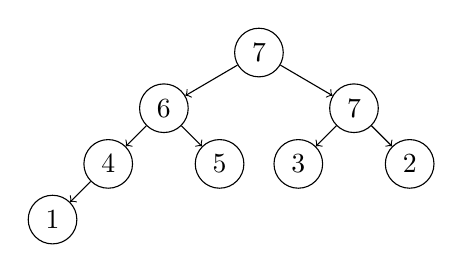
\begin{tikzpicture}[->,nodes={draw, circle}]
		\node (a8) [] {7};
		\node (a6) [below left of = a8, xshift=-0.5cm] {6};
		\node (a7) [below right of = a8, xshift=0.5cm]{7};
		\node (a4) [below left of = a6]{4};
		\node (a5) [below right of = a6]{5};
		\node (a3) [below left of = a7]{3};
		\node (a2) [below right of = a7]{2};
		\node (a1) [below left of = a4]{1};
		\draw (a8) -> (a7);
		\draw (a8) -> (a6); 
		\draw (a6) -> (a4);
		\draw (a6) -> (a5);
		\draw (a7) -> (a3);
		\draw (a7) -> (a2);
		\draw (a4) -> (a1);
		\end{tikzpicture}
	\end{center}
\end{frame}

\begin{frame}
	\frametitle{Usage}
	\begin{itemize}
		\item Priority queues
		\item Dijkstra
		\item Sorting
		\item ...
	\end{itemize}
	
	\begin{itemize}
		\item In C++: std::priority\_queue
		\item In Java: PriorityQueue
	\end{itemize}
\end{frame}
%\section{Minimum spanning trees}

In a connected graph, a spanning tree is a tree that contains all nodes
and a subset of the edges.
A minimum spanning tree is a spanning tree with minimum total length.
An example is given below:
\begin{center}
    \includegraphics[width=0.3\textwidth]{img/spanning}
\end{center}

Finding the minimum spanning tree means finding the shortest edges in total
that keep the graph connected.

\subsection{Kruskal's algorithm}

In order to construct the minimum spanning tree, Kruskal's algorithm
just picks the smallest edges first, unless adding them forms a cycle
(it would not be a tree anymore).
This is a greedy approach, and surpisingly it works.

To check if adding an edge, we can check if they belong to the same
connected component.
Since those connected components are merged together as we add edges,
they will best be represented with a union-find data structure.

The algorithm goes through the edges in increasing order of weight.
For each edge $(u,v)$, if $u$ and $v$ are in different components,
add $(u,v)$ to the tree and unite their components;
otherwise, discard the edge.

The complexity is $O(m \log m)$.

\subsection{Prim's algorithm}

The approach of Prim's algorithm is slightly different from Kruskal's.
Instead of looking at the shortest edges in the whole graph,
it begins with a starting point and picks edges to add around it.
That way it will slowly spread to the whole graph,
each time choosing the shortest edge that is in contact with the current zone.

It traverses the graph in nearly the same way as Dijkstra's algorithm,
the only difference being that Dijstra picks vertices according to their total
distance from the starting point, while for Prim only the last edge matters.
Usually, only one line needs to be changed.

When implemented with a heap, Prim's complexity is also
$O(m\log m)$.


%\section{Minimum spanning trees}

In a connected graph, a spanning tree is a tree that contains all nodes
and a subset of the edges.
A minimum spanning tree is a spanning tree with minimum total length.
An example is given below:
\begin{center}
    \includegraphics[width=0.3\textwidth]{img/spanning}
\end{center}

Finding the minimum spanning tree means finding the shortest edges in total
that keep the graph connected.

\subsection{Kruskal's algorithm}

In order to construct the minimum spanning tree, Kruskal's algorithm
just picks the smallest edges first, unless adding them forms a cycle
(it would not be a tree anymore).
This is a greedy approach, and surpisingly it works.

To check if adding an edge, we can check if they belong to the same
connected component.
Since those connected components are merged together as we add edges,
they will best be represented with a union-find data structure.

The algorithm goes through the edges in increasing order of weight.
For each edge $(u,v)$, if $u$ and $v$ are in different components,
add $(u,v)$ to the tree and unite their components;
otherwise, discard the edge.

The complexity is $O(m \log m)$.

\subsection{Prim's algorithm}

The approach of Prim's algorithm is slightly different from Kruskal's.
Instead of looking at the shortest edges in the whole graph,
it begins with a starting point and picks edges to add around it.
That way it will slowly spread to the whole graph,
each time choosing the shortest edge that is in contact with the current zone.

It traverses the graph in nearly the same way as Dijkstra's algorithm,
the only difference being that Dijstra picks vertices according to their total
distance from the starting point, while for Prim only the last edge matters.
Usually, only one line needs to be changed.

When implemented with a heap, Prim's complexity is also
$O(m\log m)$.



\end{document}